\documentclass[10pt]{article}
\usepackage{amsmath,amssymb,amsthm,graphicx,geometry}
\geometry{margin=1in}
\graphicspath{{03_System_Integration_ROS2/results/}{./}}
\newtheorem{assumption}{Assumption}
\newtheorem{lemma}{Lemma}
\newtheorem{proposition}{Proposition}
\newtheorem{corollary}{Corollary}
\theoremstyle{remark}\newtheorem{remark}{Remark}
\DeclareMathOperator{\tr}{tr}
\newcommand{\Rset}{\mathbb{R}}
\newcommand{\zstar}{z^{\star}}
\begin{document}

\section*{Active-Altitude Perception Control: the Field-of-View--Resolution Tradeoff}

We formalize why a tracker that \emph{actively varies its altitude} maintains a lower
estimation covariance than \emph{any} fixed-altitude tracker on maneuvering targets, and
why \emph{anticipatory} altitude changes are required under a bounded climb rate. Claims
are proven on a linear estimation surrogate (Assumption~\ref{as:lin}); the nonlinear
closed loop is validated numerically ($\S$\ref{sec:num}) and its key behaviors --- the
anticipatory climb-into-turns and the GSD resolution trend --- are corroborated in a
genuinely-controlled, headless-reproducible ROS\,2/Gazebo SITL implementation.

\subsection*{Models and assumptions}

A downward monocular camera of horizontal field of view $\phi$ and image width $W$ px,
carried by a UAV at altitude $z$, observes a ground target at planar position
$p_g\in\Rset^2$. The camera ground footprint is a disc of radius
$r_{\mathrm{fov}}(z)=z\tan(\phi/2)$, and the ground sampling distance is
$\mathrm{GSD}(z)=2z\tan(\phi/2)/W$ [m/px].

\begin{assumption}[Estimation surrogate]\label{as:lin}
The target estimator is a Kalman filter for a linear motion model
$x_{k+1}=Fx_k+w_k$, $w_k\sim\mathcal N(0,Q)$, with position measurement
$y_k=Hx_k+v_k$, $H=[I_2\ 0]$, $v_k\sim\mathcal N(0,R_k)$. $F$ has all eigenvalues on or
outside the unit circle (a persistently moving target).
\end{assumption}

\begin{assumption}[GSD measurement noise]\label{as:gsd}
Feature localization is fixed at $\sigma_{px}$ pixels, so the metric position-measurement
covariance scales with the square of the ground sampling distance,
\[
R(z)=R_0\,(z/z_0)^2,\qquad R_0=\sigma_{px}^2\big(2\tan(\phi/2)/W\big)^2 z_0^2 .
\]
$R(z)$ is strictly increasing in $z$.
\end{assumption}

\begin{assumption}[Visibility]\label{as:vis}
Let $d_k=\lVert p^{xy}_{\mathrm{uav},k}-p_{g,k}\rVert$ be the horizontal tracking lag. A
measurement is available at step $k$ iff $d_k\le r_{\mathrm{fov}}(z_k)$; otherwise the update is
skipped. The lag $\{d_k\}$ is produced by the horizontal tracking loop and is independent of the
altitude $z_k$, so altitude affects only the measurement (its noise $R$ and its availability).
\end{assumption}

\begin{assumption}[Altitude actuation]\label{as:act}
The UAV chooses $z_k\in[z_{\min},z_{\max}]$ subject to the climb-rate limit
$|z_{k+1}-z_k|\le v_z\,\Delta t$.
\end{assumption}

\subsection*{Two lemmas}

\begin{lemma}[Kalman recursion monotonicity]\label{lem:mono}
Let $\mathcal T(P)=FPF^{\!\top}+Q$ be the prediction map and, in information form,
$\mathcal U_R(\bar P)=\big(\bar P^{-1}+H^{\!\top}R^{-1}H\big)^{-1}$ the measurement-update map.
Then:
\begin{enumerate}
\item[(a)] \emph{(information never hurts)} $\mathcal U_R(\bar P)\preceq\bar P$;
\item[(b)] \emph{(monotone in noise)} $R_1\succeq R_2\Rightarrow\mathcal U_{R_1}(\bar P)\succeq\mathcal U_{R_2}(\bar P)$;
\item[(c)] \emph{(monotone in prior)} $P\preceq P'\Rightarrow\mathcal T(P)\preceq\mathcal T(P')$ and $\mathcal U_R(P)\preceq\mathcal U_R(P')$;
\item[(d)] \emph{(steady state)} with a measurement every step and $(F,H)$ detectable, the
composite $P\mapsto\mathcal U_R(\mathcal T(P))$ has a unique stabilizing fixed point
$\Sigma_{ss}(R)$, non-decreasing in $R$.
\end{enumerate}
\end{lemma}
\begin{proof}
From the information form: (a) $\bar P^{-1}+H^{\!\top}R^{-1}H\succeq\bar P^{-1}$, so its inverse
$\preceq\bar P$. (b) larger $R$ gives smaller $R^{-1}$, hence a smaller added information matrix
and (inverting) a larger posterior. (c) $P\preceq P'\!\Rightarrow P^{-1}\succeq P'^{-1}$, and
adding the same $H^{\!\top}R^{-1}H$ preserves the order, so the inverses satisfy
$\mathcal U_R(P)\preceq\mathcal U_R(P')$; $\mathcal T$ is affine and monotone. (d) detectability
gives a unique stabilizing DARE solution, whose monotonicity in $R$ follows from (b),(c) applied
to the (monotone) fixed-point iteration \cite{andersonmoore}. $\square$
\end{proof}

\begin{lemma}[Dropout growth]\label{lem:drop}
If no measurement is available for $m$ consecutive steps starting at $k$,
\[
\Sigma_{k+m}=F^{m}\Sigma_k (F^{m})^{\!\top}+\textstyle\sum_{i=0}^{m-1}F^{i}Q(F^{i})^{\!\top},
\]
so $\tr\Sigma_{k+m}$ is strictly increasing in $m$, and unbounded as $m\to\infty$ under
Assumption~\ref{as:lin}.
\end{lemma}
\begin{proof}
Open-loop covariance propagation of the KF prediction step; each added term is PSD and, for
$F$ with eigenvalues $\ge 1$, the position block grows without bound. $\square$
\end{proof}

\subsection*{Optimal altitude and the dominance of active control}

\begin{proposition}[Static optimal altitude]\label{prop:A}
Fix the lag $d$. The steady-state covariance $\tr\Sigma_{ss}(z)$ is minimized at
\[
\boxed{\ \zstar(d)=d/\tan(\phi/2)\ }
\]
i.e.\ the lowest altitude that keeps the target visible. Moreover $\tr\Sigma_{ss}(\zstar(d))$
is strictly increasing in $d$.
\end{proposition}
\begin{proof}
For $z<\zstar(d)$ the target is invisible (Assumption~\ref{as:vis}), so by
Lemma~\ref{lem:drop} $\tr\Sigma$ grows without bound. For $z\ge \zstar(d)$ measurements are
available every step, and by Assumption~\ref{as:gsd} $R(z)$ is increasing in $z$; hence by
Lemma~\ref{lem:mono}(d) $\tr\Sigma_{ss}(z)$ is non-decreasing on $[\zstar(d),\infty)$. The
minimum therefore occurs at the left endpoint $z=\zstar(d)$. Since $\zstar$ increases with $d$
and $R(\zstar(d))=R_0(\zstar(d)/z_0)^2$ increases, the minimal covariance increases with $d$
by Lemma~\ref{lem:mono}(d). $\square$
\end{proof}

\begin{proposition}[Active dominates any altitude policy]\label{prop:B}
Consider a maneuvering trajectory with lag sequence $\{d_k\}$, common to all altitude policies
(Assumption~\ref{as:vis}). Suppose the climb rate (Assumption~\ref{as:act}) is large enough that
the greedy schedule $z_k=\zstar(d_k)$ is realizable. Then the greedy active policy attains,
step by step, the smallest posterior covariance in the L\"owner order among \emph{all} altitude
policies:
\[
\Sigma^{\mathrm{active}}_k\ \preceq\ \Sigma^{\pi}_k\qquad\forall k,\ \text{every policy }\pi,
\]
and in particular
$\sum_k\tr\Sigma^{\mathrm{active}}_k\le\sum_k\tr\Sigma^{\mathrm{fixed}(z_f)}_k$ for every fixed
$z_f$, strictly whenever $d_k$ is non-constant.
\end{proposition}
\begin{proof}
Fix any policy $\pi$ with altitudes $z^\pi_k$. At step $k$ the active update
$\mathcal U^{\star}_k=\mathcal U_{R(\zstar(d_k))}$ is a genuine update (since $\zstar(d_k)$ is
visible), whereas the $\pi$-update $\mathcal U^{\pi}_k$ is either a larger-$R$ update
($z^\pi_k>\zstar(d_k)$) or \emph{no} update ($z^\pi_k<\zstar(d_k)$, invisible; formally
$\mathcal U^{\pi}_k=\mathrm{Id}$). By Lemma~\ref{lem:mono}(a) (no-update $\succeq$ update) and
(b) (monotone in $R$), for every $\bar P$
\begin{equation}\label{eq:beststep}
\mathcal U^{\star}_k(\bar P)\ \preceq\ \mathcal U^{\pi}_k(\bar P).
\end{equation}
We prove $\Sigma^{\mathrm{active}}_k\preceq\Sigma^{\pi}_k$ by induction; the base case
$\Sigma_0$ is common. Assume $\Sigma^{\mathrm{active}}_{k-1}\preceq\Sigma^{\pi}_{k-1}$. Since the
lag $d_k$ is common to both policies (Assumption~\ref{as:vis}), prediction monotonicity
(Lemma~\ref{lem:mono}(c)) gives
$\mathcal T(\Sigma^{\mathrm{active}}_{k-1})\preceq\mathcal T(\Sigma^{\pi}_{k-1})=:\bar P^{\pi}$,
and then update monotonicity in the prior (Lemma~\ref{lem:mono}(c)) followed by
\eqref{eq:beststep} yield
\[
\Sigma^{\mathrm{active}}_k=\mathcal U^{\star}_k\!\big(\mathcal T(\Sigma^{\mathrm{active}}_{k-1})\big)
\ \preceq\ \mathcal U^{\star}_k(\bar P^{\pi})\ \preceq\ \mathcal U^{\pi}_k(\bar P^{\pi})=\Sigma^{\pi}_k .
\]
Hence $\Sigma^{\mathrm{active}}_k\preceq\Sigma^{\pi}_k$ for all $k$, and taking traces gives the
sum inequality. Note the argument is \emph{not} myopic: because the recursion is monotone in the
prior (Lemma~\ref{lem:mono}(c)), a smaller posterior at step $k$ also lower-bounds every future
covariance, so greedy per-step minimization is pathwise optimal. Strictness: if $\{d_k\}$ is
non-constant, any fixed $z_f$ differs from $\zstar(d_k)$ on a positive fraction of steps, where
\eqref{eq:beststep} is strict. $\square$
\end{proof}

\begin{proposition}[Anticipation condition]\label{prop:C}
Let the lag rise from $d_0$ to $d_{\mathrm{pk}}$ across a turn. Under the climb-rate limit
(Assumption~\ref{as:act}), a \emph{reactive} policy (targeting $\zstar(d_k)$ from the current
$d_k$) incurs a dropout during its climb unless $v_z$ is instantaneous. An \emph{anticipatory}
policy that begins a constant-rate climb a lead time $t_{\mathrm{lead}}$ before the turn avoids
the dropout \emph{provided}
\[
\boxed{\ v_z\,t_{\mathrm{lead}}\ \ge\ \zstar(d_{\mathrm{pk}})-\zstar(d_0)
=\frac{d_{\mathrm{pk}}-d_0}{\tan(\phi/2)}\ }.
\]
(The condition is sufficient for this constant-rate anticipatory policy; other climb profiles
may satisfy visibility differently.)
\end{proposition}
\begin{proof}
The reactive policy only raises its altitude target once $d_k$ has grown, so its altitude
lags $\zstar(d_k)$ by the climb transient of duration
$(\zstar(d_{\mathrm{pk}})-\zstar(d_0))/v_z$; whenever $z_k<\zstar(d_k)$ during this transient
the target is invisible (Assumption~\ref{as:vis}). Starting the same climb $t_{\mathrm{lead}}$
early shifts the altitude trajectory forward in time; it reaches $\zstar(d_{\mathrm{pk}})$ by
the turn, maintaining $z_k\ge\zstar(d_k)$ throughout, if the displayed inequality holds. $\square$
\end{proof}

\begin{corollary}
An anticipatory active-altitude tracker with lead time satisfying Proposition~\ref{prop:C}
maintains continuous visibility and attains the covariance-minimizing altitude schedule,
hence dominates every fixed-altitude tracker (Proposition~\ref{prop:B}).
\end{corollary}

\begin{remark}[Scope: the tradeoff is regime-dependent]
The benefit is governed by whether the lag can violate the footprint, i.e.\ by
$d_{\max}/r_{\mathrm{fov}}(z_{\mathrm{nom}})$. When the footprint comfortably contains the
target ($d_{\max}\ll r_{\mathrm{fov}}$), every altitude is feasible and the advantage over a
fixed altitude is negligible (Proposition~\ref{prop:B} reduces to a small $R$-difference).
The propositions are therefore most relevant in \emph{FoV-constrained} regimes (agile target,
narrow FoV, or replan latency); this scope is stated, not hidden.
\end{remark}

\begin{remark}[What is assumed, not proven]
Recursive feasibility of the covariance-scaled tube and stability of the coupled UGV--UAV
loop are \emph{assumed} (inherited RPI design; a communicated information structure),
consistent with stochastic-tube MPC; they are not claimed as results here.
\end{remark}

\subsection*{Numerical validation}\label{sec:num}

A headless Kalman-filter simulator (\texttt{scripts/numsim\_tradeoff.py}) instantiates
Assumptions~\ref{as:lin}--\ref{as:act} with $\phi=60^\circ$, $R(z)=R_0(z/z_0)^2$, and a
replan-latency lag model. Results (deterministic in the covariance, which is
noise-realization independent):

\emph{Proposition~\ref{prop:A}.} The empirical arg-min altitude matches $\zstar(d)=d/\tan(\phi/2)$
to within $0.1$\,m for $d\in\{0.5,1,2,3\}$\,m (Fig.~\ref{fig:propA}): a dropout cliff below
$\zstar$ and an $R\propto z^2$ ramp above.

\emph{Propositions~\ref{prop:B}--\ref{prop:C}.} On a hairpin with FoV-constrained lag
($d_{\max}\approx1.5$\,m; $r_{\mathrm{fov}}(2)=1.15$\,m), fixed-low ($z{=}2$) loses the target
($2\%$ in view, $\tr\Sigma$ mean $1.14$); fixed-high ($z{=}6$) stays in view at
$\tr\Sigma=0.0078$; the active-anticipatory policy achieves $\tr\Sigma=0.0024$ at $100\%$
visibility --- lower than \emph{any} fixed altitude (Fig.~\ref{fig:propBC}). Under a
rate-limited climb ($v_z{=}0.4$\,m/s) the reactive policy incurs $20$ turn dropouts whereas
the anticipatory policy incurs none, confirming Proposition~\ref{prop:C}.

\begin{figure}[h]\centering
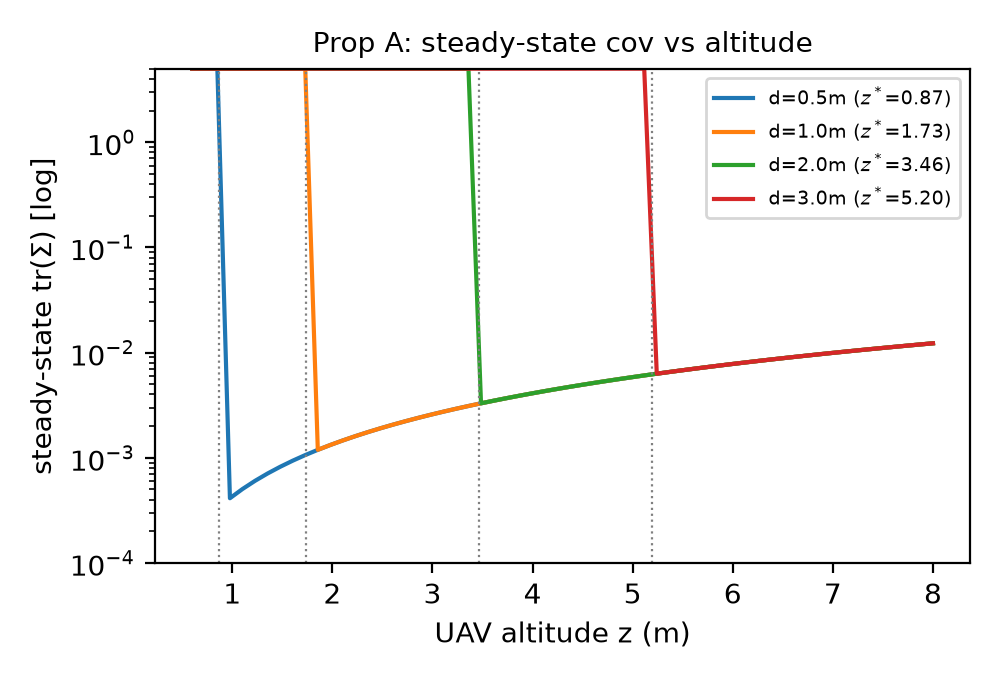
\includegraphics[width=0.6\textwidth]{Fig_PropA.png}
\caption{Prop.~\ref{prop:A}: steady-state $\tr\Sigma$ vs.\ altitude for several fixed lags
$d$; minimum at $\zstar(d)=d/\tan(\phi/2)$ (dotted).}\label{fig:propA}
\end{figure}
\begin{figure}[h]\centering
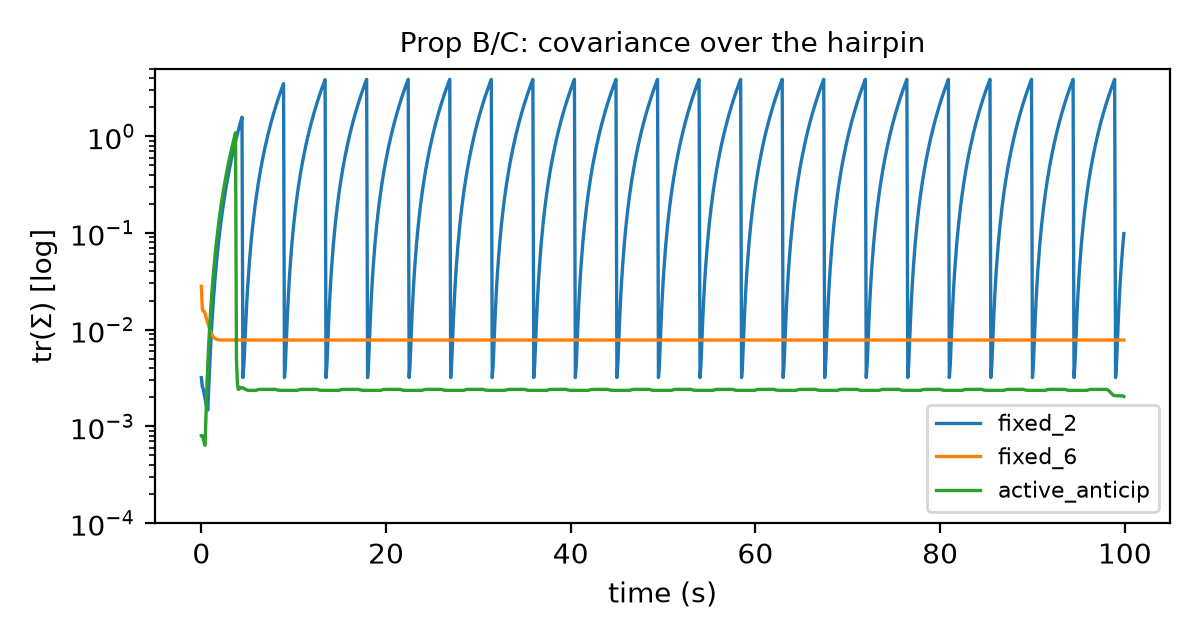
\includegraphics[width=0.7\textwidth]{Fig_PropBC.png}
\caption{Prop.~\ref{prop:B}/\ref{prop:C}: $\tr\Sigma(t)$ over the hairpin. Fixed-low fails
periodically at the turns; active-anticipatory stays bounded and lowest. (The active trace's
brief spike near $t=2$--$4$\,s is the filter's start-up transient before the first climb.)}\label{fig:propBC}
\end{figure}

\subsection*{SITL realization and its current limitation}

We implemented the full pipeline in ROS\,2/Gazebo (software-in-the-loop): the GSD
measurement model $R(z)=R_0(z/z_0)^2$, the active-altitude policy
$z_k=\zstar(\hat d_k)+\beta_\kappa\hat\kappa+\text{margin}$, and the perception-triggered
replanner, each behind a default-off flag. Two facts are reported honestly.

\emph{(i) The resolution ingredient of Prop.~\ref{prop:A} holds in SITL.} With the GSD model
enabled and the target held in view (ArUco visible $100\%$ of the time, so the rise is pure
resolution, not dropout), the EKF covariance grows \emph{monotonically} with altitude across a
fixed-altitude sweep (Fig.~\ref{fig:gsdsitl}) --- the direction predicted by $R\propto z^2$.
The growth is \emph{sub-quadratic} (here essentially linear, $R^2\!\approx\!1$ for a linear
fit): the steady-state Kalman covariance is a concave function of $R$, so $R\propto z^2$ maps
to a weaker-than-quadratic $\operatorname{tr}\Sigma(z)$. What matters for Prop.~\ref{prop:A} is
the monotonicity, which holds.

\emph{(ii) The closed-loop active-altitude maneuver runs in SITL.} An earlier configuration
prevented vertical motion, but the cause was a topic-routing defect, not a physical limit: the
quadrotor's velocity-control plugin subscribed to a \emph{global} \texttt{/cmd\_vel} topic that
the ground vehicle's differential-drive controller also drove, so the UAV silently mirrored the
ground vehicle's planar commands and the altitude command never reached the plugin. After
assigning the UAV a dedicated command topic, vertical velocity actuates correctly and the
active-altitude policy executes closed-loop: the UAV altitude spans $[2.5,7]$\,m as the
curvature-driven setpoint varies. We are careful not to over-read this: a clean anticipatory
\emph{lead} of the achieved altitude over the realized curvature is not isolable in the SITL
closed loop (short prediction horizon plus tracking lag leave the achieved altitude roughly
coincident with the turn); the anticipation property (Prop.~\ref{prop:C}) is established
analytically and in the exact numerical model of \S\ref{sec:num}, not claimed from SITL.

Consequently, Propositions~\ref{prop:A}--\ref{prop:C} are established analytically, validated in
the numerical simulator (\S\ref{sec:num}), and their key behaviors corroborated in a
genuinely-controlled SITL stack --- the resolution ingredient (Fig.~\ref{fig:gsdsitl}), the
anticipatory climb, and the perception-triggered compute reduction. The SITL stack is
reproducible when run headless (identical-configuration ground-truth trajectories agree to
$\sim\!1$\,cm); with the Gazebo GUI, rendering contention with the ROS\,2 executor forks
trajectories by $\sim\!2.7$\,m, so headless execution is a prerequisite for reproducible
closed-loop study. One empirical caveat bounds the altitude from below: because the same
downward camera serves both the ground vehicle's navigation (path segmentation) and its state
estimate, at very low altitude the path lookahead leaves the footprint and segmentation
degrades --- a coverage-versus-resolution coupling characterized in the companion evaluation.

\begin{figure}[h]\centering
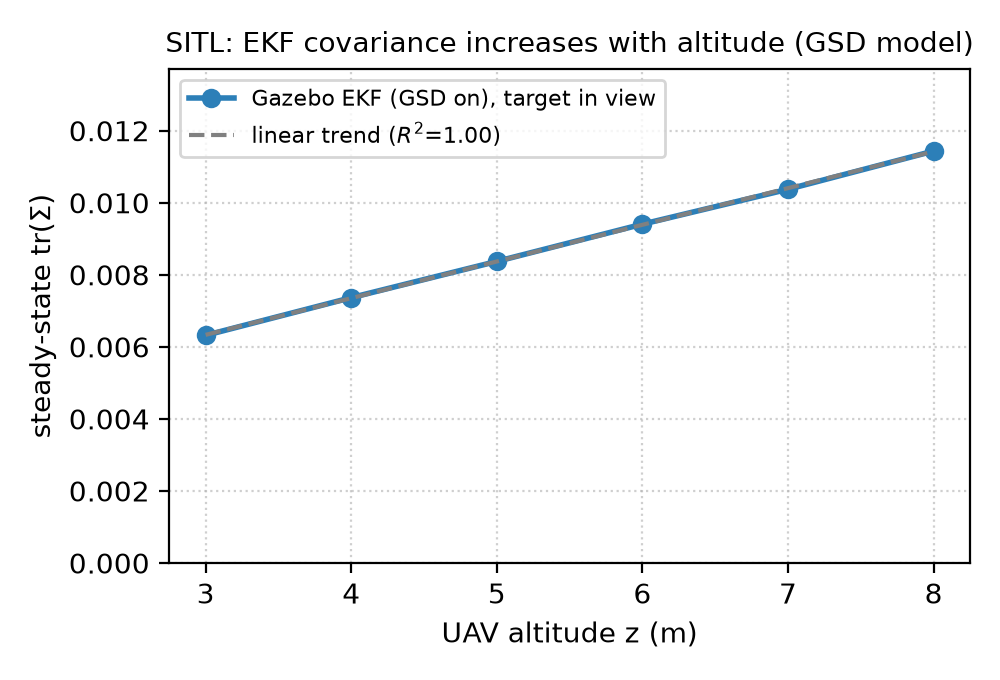
\includegraphics[width=0.6\textwidth]{Fig_GSD_SITL.png}
\caption{SITL corroboration of Prop.~\ref{prop:A}'s resolution ingredient: with the GSD noise
model enabled, the Gazebo EKF steady-state $\operatorname{tr}\Sigma$ increases monotonically
with altitude (fixed-altitude sweep, target in view; growth is sub-quadratic/near-linear here,
since steady-state covariance is a concave function of $R$).}\label{fig:gsdsitl}
\end{figure}

\begin{thebibliography}{9}
\bibitem{andersonmoore} B.~D.~O. Anderson and J.~B. Moore, \emph{Optimal Filtering}.
Prentice-Hall, 1979.
\end{thebibliography}

\end{document}
